\documentclass[../main.tex]{subfiles}
\begin{document}
\section{Red and White}
  When trying to locate Wally, one of his most prevalent features is his red and white jumper.
  Few other elements of the puzzles use the colour scheme of red and white, and less use red and white stripes.
  Finding regions with red and white stripes is one of the most immediate ways to identify Wally.

  \subsection{Implementation}
    Regions with red and white stripes can be found using a few simple techniques.
    Here, we find two masks (arrays with binary values) that describe the location of sufficiently red and white regions in the image.
    The term sufficiently is used, as defining 'red' and 'white' is not a simple task for a computer.
    The function \texttt{get\_colour\_in\_image}, discussed in section \ref{function_getcolinimg}, covers the issues with colour definition.

    Once the masks have been created, they are vertically blurred using a Gaussian blur.
    This is done so that when the two masks are multiplied together, there will be non-zero values found in overlapping areas.
    Figure \ref{rw_example} shows this graphically.
    \begin{figure}[H]
      \centering
      \begin{subfigure}[B]{0.3\textwidth}
        \centering
        
\includegraphics[height=0.8\textwidth]{rw.pdf}
        \caption{Red and White Stripes}
      \end{subfigure}
      \begin{subfigure}[B]{0.3\textwidth}
        \centering
        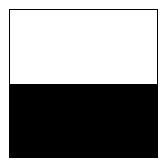
\includegraphics[height=0.8\textwidth]{rw1.pdf}
        \caption{White Mask}
      \end{subfigure}
      \begin{subfigure}[B]{0.3\textwidth}
        \centering
        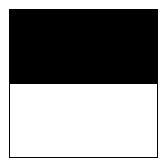
\includegraphics[height=0.8\textwidth]{rw2.pdf}
        \caption{Red Mask}
      \end{subfigure}

      \begin{subfigure}[B]{0.3\textwidth}
        \centering
        
\includegraphics[height=0.8\textwidth]{rw3.pdf}
        \caption{White Mask + Blur}
      \end{subfigure}
      \begin{subfigure}[B]{0.3\textwidth}
        \centering
        
\includegraphics[height=0.8\textwidth]{rw4.pdf}
        \caption{Red Mask + Blur}
      \end{subfigure}
      \begin{subfigure}[B]{0.3\textwidth}
        \centering
        
\includegraphics[height=0.8\textwidth]{rw5.pdf}
        \caption{Red and White blurs}
        \label{rw_stripe_ex}
      \end{subfigure}
      \caption{Example of finding red and white striped regions}
      \label{rw_example}
    \end{figure}
    The multiplication now describes regions that have red and white regions of colour that are above each other.
    As seen in figure \ref{rw_stripe_ex}, the region found may not encompass the entire area desired.
    This is solved by blurring the located stripe, making a combined region with nearby stripes.
    The regions are then identified using the \texttt{find\_region\_from\_mask} function.
  \subsection{Weaknesses}
    Finding Wally by his stripes is not wholly reliable.
    Although Wally is one of the few characters to wear red and white, he is not the only one.
    A good example of this is Wenda, figure \ref{justwenda}, who wears a similar jumper.
    Furthermore, objects in the image regularly have a red and white motif, such as skirts, umbrellas and cakes.
    Without user intervention, it is hard to prioritise results based solely on this information.
    One method is to identify the largest regions of red and white stripes in the image as most likely to be Wally.
    This is often incorrect because of the presence of large red and white objects, see figure \ref{rws_fail_small}.

    \begin{figure}[H]
      \centering
      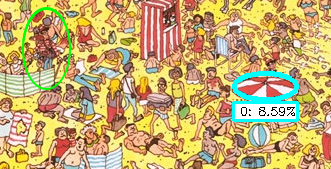
\includegraphics[width=0.8\textwidth]{results/redandwhitestripes_fail_small}
      \caption[
          Fail case for the `Red and White' pattern
        ]{
        The Red and White Stripes pattern failing to find Wally.
        The blue ring indicates the top result (an umbrella).
        The green ring indicates Wally's actual location, which is not even ranked in the top 100 results.
      }
      \label{rws_fail_small}
    \end{figure}

    One way to mitigate this is to remove 'horizontal' matches from the vertically blurred mask.
    Wally is normally found standing upright, and so his jumper normally is striped vertically.
    Horizontally stripes are unlikely to be from potential Wallys, so they are removed from the search.
    This involves repeating the same techniques required to find the regions originally, but with a horizontal blur.
    Pixels that match the horizontal blur can be removed from the original mask, preventing their inclusion in the region detection.

    Good values for the blur used for merging nearby regions are dependent on the size of Wally's stripes.
    If the value is too small, Wally's jumper as a whole is never located.
    Too large and too many incorrect regions are included in the definition of Wally's jumper.
    The size of Wally's stripes are not a known property, so a guess must be made as to a good value.
    One way of doing this is by estimating the average line width of the image, and extrapolating the size of stripes from there.
    For low resolution images, however, the ratio of stripe size to line width varies wildly, making it hard to estimate correct values.
    
  \subsection{Testing}
    \begin{figure}[H]
      \centering
      \begin{subfigure}[B]{0.4\textwidth}
        \centering
        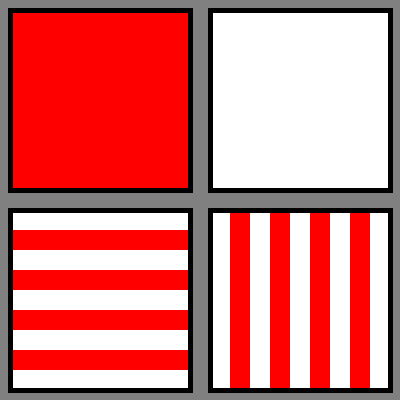
\includegraphics[width=0.9\textwidth]{rw_test1} 
        \caption{R\&W test 1}
      \end{subfigure}
      \begin{subfigure}[B]{0.4\textwidth}
        \centering
        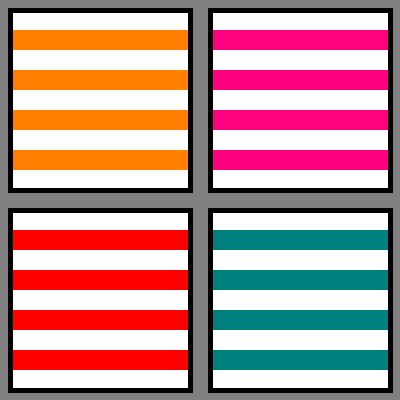
\includegraphics[width=0.9\textwidth]{rw_test3} 
        \caption{R\&W test 2}
      \end{subfigure}
      \begin{subfigure}[B]{0.4\textwidth}
        \centering
        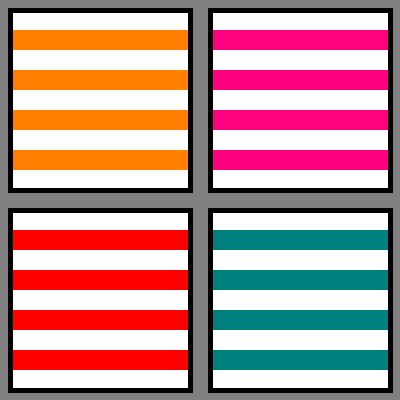
\includegraphics[width=0.9\textwidth]{rw_test3} 
        \caption{R\&W test 3}
      \end{subfigure}
      \begin{subfigure}[B]{0.4\textwidth}
        \centering
        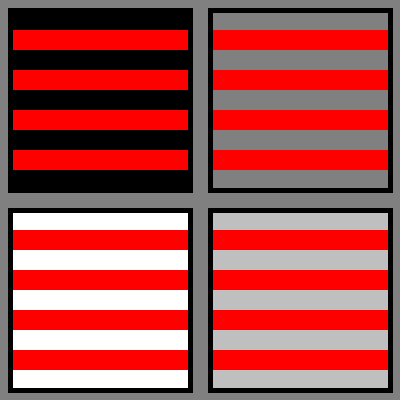
\includegraphics[width=0.9\textwidth]{rw_test4} 
        \caption{R\&W test 2}
      \end{subfigure}
      \caption{Test images used to check the red and white pattern}
    \end{figure}
  \subsection{Parallelism}
    Finding Wally's stripes is very parallelisable.
    The image can be split into parallel subimages to find the red and white masks.
    The vertical blurring only needs a small amount of information from any vertical neighbour, due to the vertical blurring.
    Choosing to break the image up vertically avoids this entirely.
    Similarly, the multiplication can be done on subimages.
    Finding the regions requires more inter-thread interaction.
    Each thread can calculate the regions for it's own subimage.
    It must then find out if it's regions are equivalent to regions in another thread.
    This can be done by sending the top row to the process above it, and the left column to the process left of it.
    By comparing the two regions a halo element is assigned, the equivalence between threads can be established.
    Figure \ref{parrregionfind} displays this graphically.
    \begin{figure}[H]
      \centering
      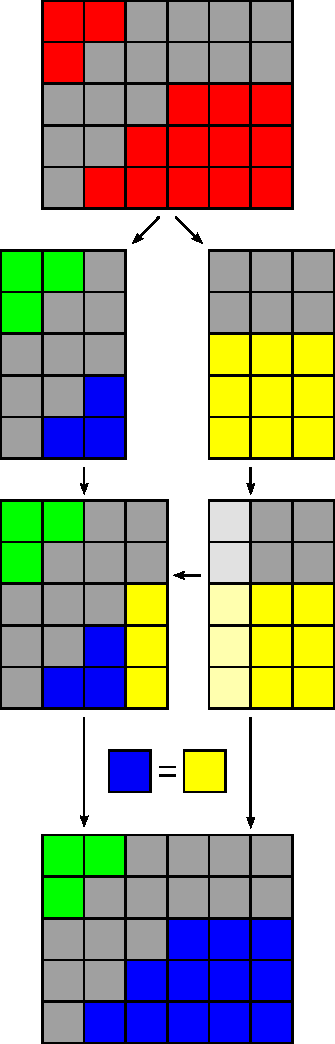
\includegraphics[width=0.2\textheight]{parallel_region}
      \caption[
          Graphic description of parallel region detection
        ]{
        A diagram explaining parallel region detection.
        The initial image is split into two sections, and each region inside the subimage is given a unique id.
        One thread sends halo data to the other, which then calculates what threads are the equivalent.
        The main image is then put back together, with the parallel region equivalences applied.
      }
      \label{parrregionfind}
    \end{figure}
    \biblio
    
\end{document}
